% Generated by Sphinx.
\def\sphinxdocclass[english]{xmosmodern}
\documentclass[  document]{xmosmodern}
\usepackage[utf8]{inputenc}
\DeclareUnicodeCharacter{00A0}{\nobreakspace}

\usepackage{longtable}



\title{Serial to Ethernet (S2E) bridging application quickstart guide}
\date{June 06, 2014}
\author{}
\newcommand{\sphinxlogo}{}
\newcommand{\releasename}{Release}
\usepackage{xsphinx}
\usepackage{threeparttable}
\usepackage{fancyvrb}
\usepackage{indent}
\renewcommand\bfcode\textbf
\renewcommand\bf\textbf
\graphicspath{{./}{./images/}}
\makeindex

\newcommand\PYGZat{@}
\newcommand\PYGZlb{[}
\newcommand\PYGZrb{]}

\setlength{\emergencystretch}{8em}
\FourDigitsInTocSection
\start

\maketitle
\pretoc
\phantomsection\label{quickstart::doc}

%last summary
\begin{inthisdocument}
\item \nameref{quickstart:serial-to-ethernet-s2e-bridging-application-quickstart-guide}
\item \nameref{quickstart:hardware-setup}
\item \nameref{quickstart:import-and-build-the-application}
\item \nameref{quickstart:flash-the-web-pages-and-device-configuration}
\item \nameref{quickstart:run-the-application}
\item \nameref{quickstart:next-steps}
\end{inthisdocument}


% NON-FULLWIDTH SECTION


This application serves as a reference design to demonstrate bridging between Ethernet and serial communication devices.
Some features of this application are:
\begin{itemize}
\item   10/100 Mbit Ethernet port

\item   Supports up to 8 serial ports (UARTs) with baud rates up to 115200 at standard UART configuration settings

\item   Webserver to facilitate dynamic UART configuration

\item   Telnet server to support data transfer via a telnet socket associated with each UART

\item   Device discovery and IP configuration management of multiple Serial to Ethernet (S2E) devices in the network

\item   Flash memory storage and retrieval for device settings such as IP, UART configuration and web pages

\item   CMOS/TTL level and RS232 level communication for UARTs

\end{itemize}




% NON-FULLWIDTH SECTION
\section{Host computer setup}
\label{quickstart:serial-to-ethernet-s2e-bridging-application-quickstart-guide}\label{quickstart:host-computer-setup}

A computer with:
\begin{itemize}
\item   With a spare Ethernet port

\item   Internet browser (Internet Explorer, Chrome, Firefox, etc...)

\item   Download and install xTIMEcomposer studio (v13.0.0 or later) from XMOS xTIMEcomposer downloads webpage

\item   A spare USB port for XTAG debug

\item   A spare DB9 port (an additional USB port may be used for serial to USB adapter if DB9 port is not available)

\end{itemize}



For serial-telnet data communication demo, the following are required in addition to the above:
\begin{itemize}
\item   A null serial cable to DB-9 connector. The cable will need a cross over between the UART RX and TX pins at each end.

\item   If the computer does not have a DB-9 connector slot, any USB-UART cable can be used. For the demo, we use BF-810 USB-UART adapter

\end{itemize}



(\verb`http://www.bafo.com/products/accessories/usb-devices/bf-810-usb-to-serial-adapter-db9.html`).
* A suitable terminal client software. For MAC users, try SecureCRT (\verb`http://www.vandyke.com/download/securecrt/`) and for Linux users, try cutecom (\verb`http://cutecom.sourceforge.net/`). We use hercules client (\verb`http://www.hw-group.com/products/hercules/index_en.html`) on a Windows platform for the demo.



% NON-FULLWIDTH SECTION
\section{Hardware setup}
\label{quickstart:hardware-setup}

Required sliceKIT units:
\begin{itemize}
\item   xCORE General Purpose (L-series) sliceKIT core board 1V2 (XP-SKC-L2)

\item   Ethernet sliceCARD 1V1 (XA-SK-E100)

\item   Multi UART sliceCARD (XA-SK-UART-8)

\item   xTAG-2 debug adapter and sliceKIT connector (xTAG-2 and XA-SK-XTAG2)

\end{itemize}



Setup:
\begin{itemize}
\item   Connect the \verb`XA-SK-XTAG2` adapter to the \verb`XP-SKC-L2` sliceKIT core board.

\item   Ensure the \emph{XMOS Link} switch is at \emph{ON} position on the \verb`XA-SK-XTAG2` adapter.

\item   Connect \verb`XTAG2` to \verb`XSYS` side (\verb`J1`) of the \verb`XA-SK-XTAG2` adapter.

\item   Connect the \verb`XTAG2` to your computer using a USB cable.

\item   Connect the \verb`XA-SK-UART-8` Multi UART sliceCARD to the \verb`XP-SKC-L2` core board's \verb`SQUARE` (indicated by a white colour square) slot.

\item   Connect the \verb`XA-SK-E100` Ethernet sliceCARD to the \verb`XP-SKC-L2` core board's \verb`TRIANGLE` (indicated by a white colour triangle) slot.

\item   Using an Ethernet cable, connect the other side of \verb`XA-SK-E100` Ethernet sliceCARD to your computer's Ethernet port.

\item   Connect the 12V power supply to the core board and switch it ON.

\end{itemize}

\begin{figure}[h]
\begin{sidecaption}{Hardware setup}

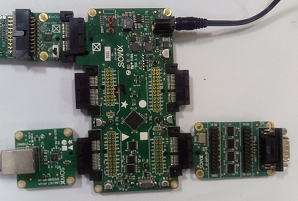
\includegraphics[width=\ScaleIfNeeded]{hardware_setup.png}
\end{sidecaption}\end{figure} \DocumentFooterFix



% NON-FULLWIDTH SECTION
\section{Import and build the application}
\label{quickstart:import-and-build-the-application}

Importing the \verb`serial to ethernet` reference application:
\begin{itemize}
\item   Open the xTIMEcomposer studio.

\item   Open the \emph{Edit} perspective (Window -\textgreater{} Open Perspective -\textgreater{} XMOS Edit).

\item   Access the \emph{Import} option either by right clicking in the project explorer window or through File -\textgreater{}Import menu

\item   Click \emph{Import} option (Import -\textgreater{} General -\textgreater{} Existing Projects into Workspace and click Next).

\item   Choose \emph{Select archive file} option and click \emph{Browse} button.

\item   Select s2e reference design release package and click \emph{Finish} button

\item   The application is called as \emph{app\_serial\_to\_ethernet} in the \emph{Project Explorer} window.

\end{itemize}



Building the \verb`serial to ethernet` application:
\begin{itemize}
\item   Click on the \emph{app\_serial\_to\_ethernet} item in the \emph{Project Explorer} window.

\item   Click on the \emph{Build} (indicated by a `Hammer' picture) icon.

\item   Check the \emph{Console} window to verify that the application has built successfully.

\end{itemize}




% NON-FULLWIDTH SECTION
\section{Flash the web pages and device configuration}
\label{quickstart:flash-the-web-pages-and-device-configuration}

To flash the web pages and device configuration using xTIMEcomposer studio:
\begin{itemize}
\item   In the \emph{Project Explorer} window, locate the \emph{app\_serial\_to\_ethernet.xe} and \emph{web\_data.bin} in the (app\_serial\_to\_ethernet -\textgreater{} bin)

\item   Right click on \emph{app\_serial\_to\_ethernet.xe} and click on (Flash As -\textgreater{} Flash Configurations...).

\item   In the \emph{Flash Configurations} window, double click the \emph{xCORE Application} to create a new flash configuration.

\item   Navigate to \emph{XFlash Options} tab and apply the following settings:
\begin{itemize}
\item   Check \emph{Boot partition size (bytes):} and its value as 0x10000

\item   \emph{Other XFlash Options:} as \verb`--data bin/web_data.bin`

\end{itemize}


\item   Click on \emph{Apply} and then \emph{Flash} to the XMOS device.

\item   Check the \emph{Console} window to verify flashing progress.

\end{itemize}




% NON-FULLWIDTH SECTION
\section{Run the application}
\label{quickstart:run-the-application}

To run the application using xTIMEcomposer studio:
\begin{itemize}
\item   In the \emph{Project Explorer} window, locate the \emph{app\_serial\_to\_ethernet.xe} in the (app\_serial\_to\_ethernet -\textgreater{} Binaries).

\item   Right click on \emph{app\_serial\_to\_ethernet.xe} and click on (Run As -\textgreater{} xCORE Application).

\item   In the \emph{Run Configurations} window, double click the \emph{xCORE Application} to create a new xCORE application launch configuration.

\item   A \emph{Select Device} window appears.

\item   Select \emph{XMOS XTAG-2 connected to L1} and click \emph{Apply}.

\item   Click \emph{Run} and check the \emph{Console} window for any messages.

\end{itemize}



Demo:
\begin{itemize}
\item   The following message appears in the \emph{Console} window of the xTIMEcomposer studio:

\vspace{-5pt}\begin{minipage}{\linewidth}
\begin{lstlisting}[]
Address: 0.0.0.0
Gateway: 0.0.0.0
Netmask: 0.0.0.0
\end{lstlisting}
\end{minipage}


\item   At this point, the XMOS device is trying to acquire an IP address in the network. Wait for some time (approximately 20 seconds) for the following message to appear in the \emph{Console} window. Note, the IP address may be different based on your network:

\vspace{-5pt}\begin{minipage}{\linewidth}
\begin{lstlisting}[]
ipv4ll: 169.254.161.178
\end{lstlisting}
\end{minipage}


\item   Open a web browser (Firefox, etc...) in your host computer and enter the above IP address in the address bar of the browser. It opens a web page as hosted by the webserver running on the XMOS device.

\end{itemize}

\begin{figure}[h]
\begin{sidecaption}{Page hosted by webserver to support UART configuration}

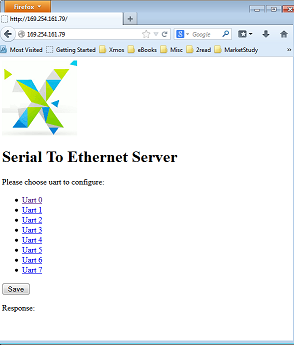
\includegraphics[width=\ScaleIfNeeded]{webpage.png}
\end{sidecaption}\end{figure} \DocumentFooterFix
\begin{itemize}
\item   To change the configuration of a UART via web page, click on any UART, say UART 1. It opens a new page for configuring the selected UART 1.

\item   Observe the \emph{Telnet Port} value for the selected UART. This is the telnet port number on which the UART1 is bridged.

\item   Alter the \emph{Baud Rate} settings from \emph{115200} to \emph{57600} by choosing this value from the drop box.

\item   Click on \emph{Set} button and verify the \emph{Response:} value is populated as \emph{Ok}.

\item   Click \emph{Back to main config page} link to go back to the home page and verify the modified UART settings are intact by clicking on the same UART 1.

\item   On the main page, click on \emph{Save} button to store any modified UART settings onto the flash.

\end{itemize}

\begin{figure}[h]
\begin{sidecaption}{Modifying UART configuration via web page}

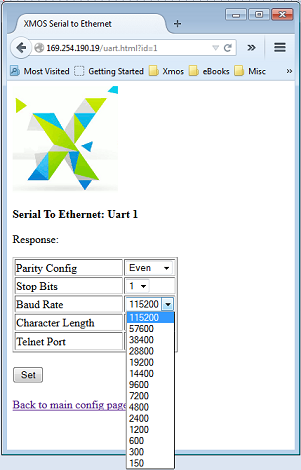
\includegraphics[width=\ScaleIfNeeded]{modify_uart_configuration.png}
\end{sidecaption}\end{figure} \DocumentFooterFix


Serial-Telnet data communication demo:


This demo showcases the data bridging between Ethernet and serial devices. Data from the Serial console (UART) is sent to the corresponding telnet socket associated with the UART and vice versa. In order to run this demo, follow the below instructions.


In addition to the above hardware setup
\begin{itemize}
\item   Connect a null serial cable to DB-9 connector on Multi UART sliceCARD.

\item   Connect other end of cable to DB-9 connector slot on the host or USB-UART adapter.

\item   Identify the serial (COM) port number provided by the Host or \emph{USB to UART} adapter and open a suitable terminal client software for the selected COM port (if required, refer to the documentation of the selected application).

\item   Configure the host COM port console settings; sample settings while using Hercules client should be as follows:

\end{itemize}


\begin{tabular}{ll}
\Toprule
Parameter & Value\\
Baud rate & 115200\\
Data size & 8\\
Parity & Even\\
Handshake & off\\
Mode & Free\\
\bottomrule
\end{tabular}



The Transmit End-of-Line character should be set to \emph{CR} (other options presented will probably be \emph{LF} and \emph{CRLF}). In hercules, this setting is achieved by right clicking on \emph{Received/Sent Data} text box, select \emph{Transmit EOL}, select \emph{CR(Mac)} option


If any other terminal console is used, and has any additional settings, following values are used:
.. list-table:

\vspace{-5pt}\begin{minipage}{\linewidth}
\begin{lstlisting}[,resetmargins=true]
* - Parameter
  - Value
* - Stop bit
  - 1
* - hardware flow control
  - none
\end{lstlisting}
\end{minipage}

\begin{itemize}
\item   Click on \emph{Open} to open the COM port.

\item   Now, in order to establish a telnet connection to the above serial connection, open a telnet client application (On Windows, open another instance of the Hercules application, select \emph{TCP Client} tab)

\item   Configure the telnet client application with ip address as XMOS device address. Key in the port number as \emph{46} in order to connect to the UART0.

\item   Click \emph{Connect} so that the telnet client connects to the telnet server running on the S2E device. Observe a welcome message \emph{Welcome to serial to ethernet telnet server demo! This server is connected to uart channel 0} appears on the client application console.

\end{itemize}

\begin{figure}[h]
\begin{sidecaption}{Screenshot of two Hercules application instances for a serial console and a telnet client}

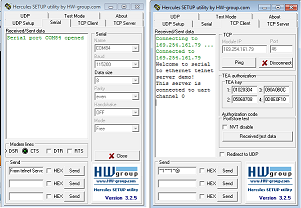
\includegraphics[width=\ScaleIfNeeded]{terminal_clients.png}
\end{sidecaption}\end{figure} \DocumentFooterFix
\begin{itemize}
\item   Key in some data from the serial console and observe the data is displayed on the telnet console.

\item   Now send some data from the telnet console and verify the same data on the serial console.

\item   Explore the terminal client options to transfer a file in both directions and observe the duplex data transfer in action.

\end{itemize}

\begin{figure}[h]
\begin{sidecaption}{Data communication between a telnet socket and a serial console (UART)}

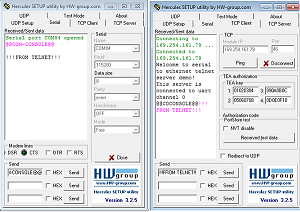
\includegraphics[width=\ScaleIfNeeded]{data_communication.png}
\end{sidecaption}\end{figure} \DocumentFooterFix



% NON-FULLWIDTH SECTION
\section{Next steps}
\label{quickstart:next-steps}\begin{itemize}
\item   Connect two or more USB-UART adapters to the host and Multi UART sliceCARD. Open the terminal client applications for the correct configuration as detailed in the above \emph{Serial-Telnet data communication demo}. Test the data communication between the connected UARTs and their corresponding Telnet sockets.

\item   Detach xTAG-2 debug adapter and sliceKIT connector from xCORE General Purpose (L-series) sliceKIT core board. Connect Ethernet sliceCARD to a spare Ethernet port of the router. If your platform is a MAC or a linux host, navigate to \verb`sw_serial_to_ethernet -> tests -> udp_test_server` and run the udp\_server.py python script (python udp\_server.py). If you are using a Windows host, download \emph{Serial\_to\_Ethernet\_UDP\_test\_server} package and extract its contents to a directory. Navigate to (udp\_test\_server -\textgreater{} windows -\textgreater{} udp\_server.exe), right-click on udp-server.exe and run as Administrator. The script displays the selected network adapter on the console. If there are multiple network adapters on your host, ensure the ip address used by the script corresponds to the one used by your network adapter connected to the router. Now, select option \verb`1` to discover the S2E devices available on the network. Look at the S2E device ip address as displayed by the script. Open a web page or test Telnet-UART data communication using ip of the S2E device. Select other choices to change ip configuration settings of the S2E device(s).

\item   Take a look at the \verb`http://xcore.github.io/sw_serial_to_ethernet` for a more detailed documentation on using various features, design and programming guide for the application.

\end{itemize}





\finish
